%*****************************************
\chapter{Antecedentes}\label{ch:antecedentes}
%*****************************************

En este capítulo se discute brevemente el fenómeno biológico que se quiere entender a través de modelación computacional. Posteriormente se discuten un modelo de red Booleana de tres nodos que se usó para ganar entendimiento de cómo transformar un modelo discreto en uno semicontinuo, así como del modelo de la vía de señalización basado en funciones discretas. Este último modelo es un antecedente directo del semicontinuo desarrollado en este trabajo.

\section{Antecedentes biol\'ogicos}

La fertilización es un proceso crucial para la preservación de la vida, que requiere el encuentro y fusión de los gametos. Para que este encuentro tenga lugar, el espermatozoide debe valerse de una intrincada maquinaria en su flagelo que le permita nadar en busca del óvulo. En algunas especies, el óvulo secreta una sustancia quimioatrayente que guía al esperma hacia él. En el caso particular del erizo de mar, esta sustancia es un decapéptido llamado \emph{speract}, el cual se une a un receptor específico en la membrana del flagelo del espermatozoide. La unión de speract con su receptor activa una red de señalización que produce oscilaciones en la concentración interna de algunos iones, de los cuales el principal es el calcio. 

La vía de señalización inducida por speract provoca la apertura de distintos canales que hiperpolarizan la membrana. A su vez, esta hiperpolarización cancela la desactivación de canales regulados por voltaje, que al abrirse despolarizan la membrana. Este proceso repetido de hiper y despolarización se ha relacionado con cambios transitorios en la curvatura del flagelo del espermatozoide que resultan en modificaciones abruptas de su trayectoria. Estos cambios de trayectoria son una parte esencial para la motilidad y reorientación del esperma. De ahí la importancia de entender los mecanismos bioquímicos que la generan. 

Las oscilaciones de \textsc{calcio intracelular} $[Ca^{2+}]_i$ se caracterizan por presentar un incremento sostenido \emph{(tónico)} y fluctuaciones superimpuestas \emph{(supratónico)}, tal como se muestra en la figura \ref{fig:fluorescencia}. Se cuenta con mediciones experimentales de la vía de señalización consistentes en añadir un marcador fluorescente al calcio. Al estimularse la vía mediante la adición de speract al medio, es posible observar dichos incrementos tónico y supratónico en la concentración de calcio. Los datos fueron obtenidos por Adán Guerrero en el laboratorio del Dr. Alberto Darszon. \citeauthor{Darszon2008} \citep{Darszon2008} y \citeauthor{Wood2007} \citep{Wood2007} presentan una descripción más detallada del tipo de técnicas experimentales usadas para la obtención de estos datos.


\begin{figure}[hbt]
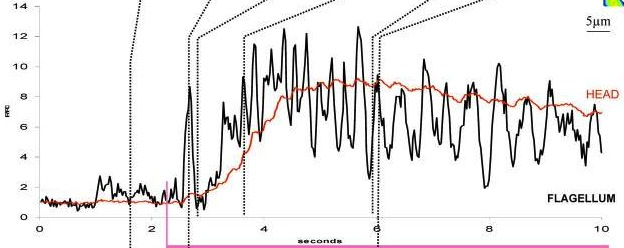
\includegraphics[width=0.9\linewidth]{gfx/maderaSperact}
\caption[Medición experimental de calcio intracelular]{Medición experimental de fluorescencia de calcio intracelular en espermatozoides. Las oscilaciones tónicas corresponden al incremento sostenido en la concentración de calcio, y tienen una forma de letra "s". Este tipo de oscilaciones se presentan tanto en la cabeza como en el flagelo del espermatozoide. En la figura, la serie en rojo corresponde a la concentración de calcio en la cabeza, mientras que los datos en color negro corresponden a la concentración de calcio en el flagelo. Las oscilaciones supratónicas se observan solamente en el flagelo y se distinguen por ser las fluctuaciones que parecen "montarse"\ sobre la curva con forma de "s". Figura modificada tomada de \citeauthor{Wood2003} \citep{Wood2003}.}\label{fig:fluorescencia}
\end{figure}


Vistos a detalle, los eventos de la vía de señalización que se muestra en la figura \ref{fig:erizobBioquimica}, inician con la unión de speract a su \textsc{receptor} $(SR)$, que interacciona con una \textsc{Guanilato Ciclasa} $(GC)$ que produce \textsc{Guanosín Monofosfato(GMP) cíclico} $(cGMP)$. El aumento en la concentración de $cGMP$ abre el canal $(KCNG)$, que es un \textsc{canal de potasio} $(K^+)$ \textsc{regulado por cGMP}. La apertura de $(KCNG)$ resulta en la hiperpolarización del \textsc{potencial de membrana} $(V)$. Como consecuencia de la hiperpolarización suceden cuatro eventos importantes: \begin{enumerate}
\item se activa un \textsc{intercambiador} $Na^+/Ca^{2+}$ $(NCE)$ que disminuye los niveles de \textsc{calcio intracelular} $[Ca^{2+}]_i$
\item se activa un \textsc{intercambiador} $Na^+/H^+$ ($NHE)$ que incrementa el \textsc{pH intracelular} $(pH_i)$
\item se activa un \textsc{canal activado por hiperpolarización y regulado por nucleótidos cíclicos} $(HCN)$
\item finalmente, la sustracción de la inactivación del \textsc{canal de Calcio dependiente de alto voltaje} $(HVA)$ y el \textsc{canal de Calcio dependiente de bajo voltaje} $(LVA)$
\end{enumerate}

\begin{figure}[hbt]
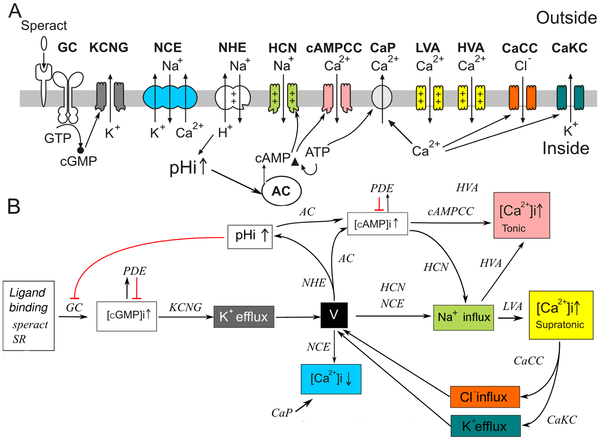
\includegraphics[width=0.9\linewidth]{gfx/redErizoBioquimica}
\caption[Red de se\~nalizaci\'on]{Red de se\~nalizaci\'on \citeauthor{Espinal2011} \citep{Espinal2011}.\ A) Componentes principales involucrados en la vía de señálización de speract. La unión de speract a su receptor en la membrana del flagelo dispara la cascada que produce cambios en $[Ca^{2+}]_i$ de dos maneras: un incremento sostenido (tónico) y fluctuaciones superimpuestas (supratónico). B) Eventos producidos por la vía de señalización.}\label{fig:erizobBioquimica}
\end{figure}

El incremento del $pH_i$ disminuye la actividad de $GC$ a la vez que activa una \textsc{adenilato ciclasa soluble} $(sAC)$, con la consecuente producción de \textsc{Adenosín Monofosfato Cíclico} $(cAMP)$. Este último estimula un \textsc{canal de calcio dependiente de cAMP} $(cAMPCC)$ y el canal $HCN$ previamente activado, lo cual tiene a repolarizar el potencial de membrana. Esta repolarización abre los canales $HVA$ y $LVA$ causando una despolarización y un incremento del $[Ca^{2+}]_i$. Finalmente, la vía de señalización se inicia de nuevo, posiblemente a través de un \textsc{canal de} $Ca^{2+}$ \textsc{dependiente de} $Cl^-$ $(CaCC)$ y un \textsc{canal de} $Ca^{2+}$ \textsc{dependiente de} $K^+$ $(CaKC)$, que se abren cuando la concentración de $[Ca^{2+}]_i$ es alta. Los mecanismos pasivos y constantes de extrusión de $Ca^{2+}$, tales como \textsc{bombas de calcio} $(CaP)$ y $NCE$, mantienen los niveles basales de $[Ca^{2+}]_i$. El mecanismo anteriormente descrito es repetido cíclicamente, generando un tren de oscilaciones de $Ca^{2+}$ que produce una secuencia repetitiva de cambios de dirección en el espermatozoide. 

\section{Antecedentes de modelos discretos}

Los modelos de red Boolena (o más generalmente, modelos discretos) son discretos en tiempo y estado, donde cada componente de una vía de señalización  bioquímica o red regulatoria genética se considera como un nodo. La red está formada por estos nodos y un conjunto de aristas, que representan el tipo de interacción existente entre cada par de nodos. Estas interacciones pueden ser de activación o de inhibición. 

En cada paso de tiempo $t$ un nodo de la red puede encontrarse en un estado $0$ ó $1$. El $0$ representa actividad basal o inactividad, mientras que el $1$ representa actividad o expresión. En general, se pueden establecer distintos niveles de expresión o actividad si se considera que los nodos puedan tomar valores discretos, i.e. $0, 1, -1, 2,$ etc.

El sistema evoluciona a través del tiempo mediante una regla de evolución. Cada nodo $i$ de la red tiene asociada una de estas reglas de evolución,  que depende de $k$ nodos reguladores de $i$, es decir, aquellos nodos que tienen una arista incidente en el nodo $i$. Si denotamos el estado del nodo $i$ en el tiempo $t$ con $\sigma_i(t)$, tenemos el mapeo discreto

\begin{equation}\label{eqn:kaufman}
\sigma_i(t+1) = F_i[\sigma_{i_1}(t), \sigma_{i_2}(t),\ldots, \sigma_{i_k}(t)]
\end{equation}

Iterando esta regla de evolución para cada nodo de la red se obtiene una descripción por pulsos de la dinámica del sistema. Cada pulso puede ser considerado como el promedio discretizado de la variable de estado de cada nodo de la red durante un intervalo de tiempo dado. Si bien el $(t+1)$ en la función de evolución se refiere a un tiempo de máquina o tiempo de simulación, es posible hacer comparaciones entre este tiempo de máquina y el tiempo de los experimentos.

Uno de los aspectos fundamentales de este tipo de modelos discretos es que cualquier configuración inicial posible de estados del sistema llega a un conjunto de configuraciones que se repiten a lo largo del tiempo tras iterar un cierto número de veces la reglas de evolución de la red. Estas configuraciones finales pueden ser puntuales, es decir, la misma configuración se repite \emph{ad eternum}; o bien cíclicas, es decir, el sistema vuelve a la misma configuración después de un cierto número de pasos de tiempo. Estas configuraciones puntuales o cíclicas se conocen como atractores. El conjunto de configuraciones iniciales que  tras una serie de pasos conocidos como transitorio terminan en un atractor se denomina cuenca de atracción.

\citeauthor{huang2005} \citep{huang2005} muestran que los atractores din\'amicos corresponden a patrones estables de expresi\'on gen\'etica que determinan estados funcionales estables de una c\'elula. En el caso del modelo de la red de se\~nalizaci\'on que se estudia en este trabajo, los atractores de la red determinan las oscilaciones estables de calcio que posibilitan la relocalizaci\'on de los espermatozoides a trav\'es de las alteraciones que el calcio induce a la curvatura del flagelo.

\subsection{Modelo discreto de tres nodos}\label{sect:3nodos}

%% ESTA SECCIóN REQUIERE UN MAJOR REWRITING :S

Con el objetivo de explorar y ganar entendimiento acerca de cómo transformar modelos discretos en modelos de Glass, se utilizó una red Booleana de tres nodos que había sido estudiada previamente por \citeauthor{Reka3Nodos2010}. En ese trabajo se caracteriza por completo el comportamiento de dicha red discreta. Este modelo discreto es mostrado en la figura \ref{fig:red3reka}.

\begin{figure}[hbt]
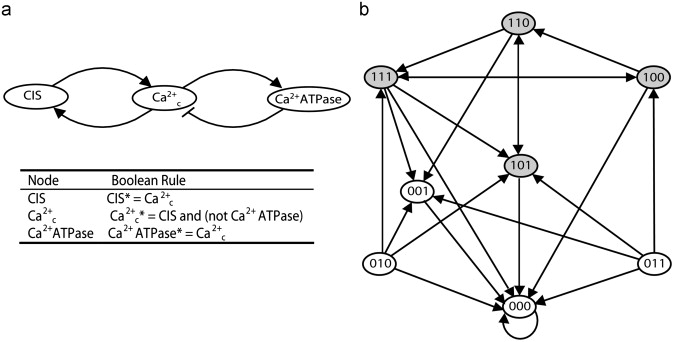
\includegraphics[width=0.9\linewidth]{gfx/red3nodos}
\caption[Modelo Booleano de 3 nodos]{Modelo Booleano de 3 nodos de \citeauthor{Reka3Nodos2010} \citep{Reka3Nodos2010}.\ a) Reglas L\'ogicas.\ b) Estados posibles de la red.}\label{fig:red3reka}
\end{figure}


Si bien este modelo no esta relacionado con la red de señalización discutida en esta tesis, el hecho de contar con pocos nodos sirvió como un buen punto de partida para transformar un modelo Booleano en uno de ecuaciones de Glass.

\subsection{Modelo discreto de la vía de señalización inducida por speract}\label{sect:erizo}


\citeauthor{Espinal2011} \citep{Espinal2011} presentan un modelo discreto en tiempo y estado para la vía de señalización inducida por speract en el flagelo del esperma de erizo de mar. En ese trabajo, dieciocho de los veintidos nodos toman valores de estado $0$ ó $1$, mientras que los cuatro nodos restantes tienen un valor de estado ternario, es decir, cada uno de estos nodos puede encontrarse en el estado $0$, $1$ ó $2$. Esta extensión a tres valores posibles es necesaria para capturar los estados posibles en los que se puede encontrar un componente de la red, véase la figura \ref{fig:erizoModelo}.

\begin{figure}[hbt]
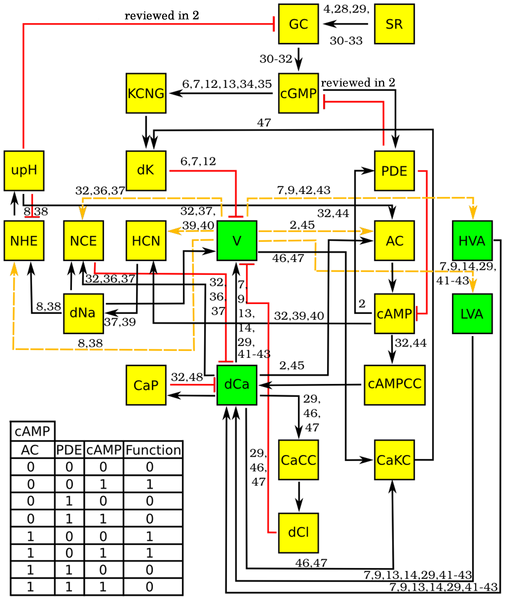
\includegraphics[width=0.9\linewidth,height=10cm]{gfx/redErizoModelo}
\caption[Modelo Discreto de la red de se\~nalizaci\'on]{Modelo Discreto de la red de se\~nalizaci\'on \citeauthor{Espinal2011} \citep{Espinal2011}.\ Los cuadros amarillos y verdes indican nodos binarios y ternarios, respectivamente. Las flechas negras indican activación, las líneas rojas inhibición y las flechas amarillas pueden representar activación o inhibición, dependiendo del valor del nodo de voltaje $(V)$. Los números sobre las flechas corresponden a las referencias con las que \citeauthor{Espinal2011} \citep{Espinal2011} construyeron la red y sustentan cada interacción. A manera de ejemplo, la función reguladora o tabla de verdad del nodo de $cAMP$ se muestra en la esquina inferior izquierda. Las primeras 3 columnas en esta tabla contienen todos los valores posibles de activación de los reguladores de $cAMP$, $(AC,\ PDE,\ cAMP)$; la cuarta columna muestra los valores para la función que corresponden a cada combinación de los reguladores.}\label{fig:erizoModelo}
\end{figure}

En el trabajo citado, se determina que este modelo llega a dos configuraciones cíclicas o atractores, uno de período cuatro y otro de período ocho. Estos atractores se relacionaron con las mediciones experimentales de fluorescencia de calcio en el flagelo del espermatozoide. El atractor de período cuatro, al cual convergen el $80\%$ de las configuraciones iniciales posibles, puede entenderse entonces como una descripción promedio discretizada en cuatro intervalos de tiempo del modelo que tienen relación con una oscilación de calcio, es decir, cuatro unidades de tiempo del modelo discreto se relacionan con la duración de una oscilación de calcio intracelular en las mediciones experimentales.

\begin{figure}[hbt]
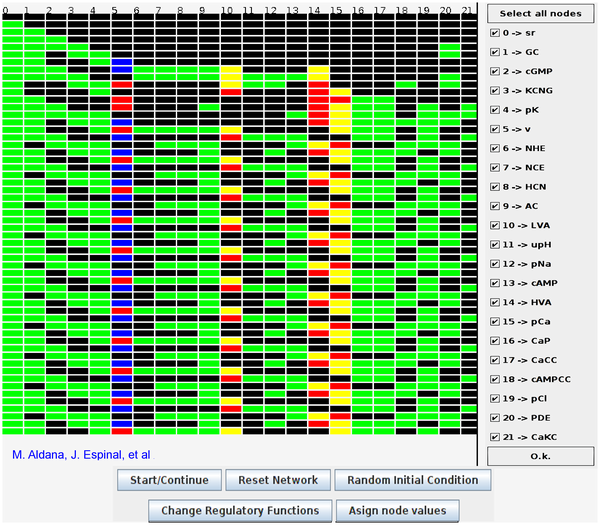
\includegraphics[width=0.9\linewidth%,height=10cm
]{gfx/appletErizo}
\caption[Applet del Modelos Discreto]{Applet del Modelo Discreto de la red de se\~nalizaci\'on \citeauthor{Espinal2011} \citep{Espinal2011}.\ Serie temporal de los patrones de activación de la red de señalización bajo diferentes condiciones. En cada caso, los nodos están en el eje horizontal y el tiempo en el eje vertical. Para los nodos binarios, el negro representa el estado \emph{apagado}, verde \emph{encendido}. Los nodos $10$ y $14$, correspondientes al $HVA$ y $LVA$, el negro es un estado inactivo, el amarillo corresponde a un canal cerrado y el rojo a un canal abierto. El nodo 5, correspondiente al potencial de membrana $V$ es negro para un potencial en reposo, azul para la hiperpolarización y rojo para la repolarización. El nodo 15 $(dCa)$, correspondiente al $Ca^{2+}$ es amarillo para indicar el incremento tónico, rojo para el incremento supratónico y negro para indicar estado basal. Como puede observarse, tras un transitorio la red llega a un atractor de período 4. Se muestra el comportamiento del especímen silvestre (wt).
El applet fue desarrollado por el Dr. Maximino Aldana y se encuentra disponible en \url{http://www.fis.unam.mx/research/seaurchin/discrete/}. Este applet permite explorar de manera interactiva distintas condiciones iniciales, cambiar las reglas lógicas así como observar el comportamiento de la red en ausencia de algunos nodos.}\label{fig:appletErizo}
\end{figure}
%%(Insertar figura que explique esto).
%%Discusión aquí de algunos de los resultados del modelo discreto.
